%%%%%%%%%%%%%%%%%%%%%%%%%%%%%%%%%%%%%%%%%
% Beamer Presentation
% LaTeX Template
% Version 1.0 (10/11/12)
%
% This template has been downloaded from:
% http://www.LaTeXTemplates.com
%
% License:
% CC BY-NC-SA 3.0 (http://creativecommons.org/licenses/by-nc-sa/3.0/)
%
%%%%%%%%%%%%%%%%%%%%%%%%%%%%%%%%%%%%%%%%%

%----------------------------------------------------------------------------------------
%	PACKAGES AND THEMES
%----------------------------------------------------------------------------------------

\documentclass{beamer}

\mode<presentation> {

% The Beamer class comes with a number of default slide themes
% which change the colors and layouts of slides. Below this is a list
% of all the themes, uncomment each in turn to see what they look like.

%\usetheme{default}
%\usetheme{AnnArbor}
%\usetheme{Antibes}
%\usetheme{Bergen}
%\usetheme{Berkeley}
%\usetheme{Berlin}
%\usetheme{Boadilla}
%\usetheme{CambridgeUS}
%\usetheme{Copenhagen}
%\usetheme{Darmstadt}
%\usetheme{Dresden}
%\usetheme{Frankfurt}
%\usetheme{Goettingen}
%\usetheme{Hannover}
%\usetheme{Ilmenau}
%\usetheme{JuanLesPins}
%\usetheme{Luebeck}
\usetheme{Madrid}
%\usetheme{Malmoe}
%\usetheme{Marburg}
%\usetheme{Montpellier}
%\usetheme{PaloAlto}
%\usetheme{Pittsburgh}
%\usetheme{Rochester}
%\usetheme{Singapore}
%\usetheme{Szeged}
%\usetheme{Warsaw}

% As well as themes, the Beamer class has a number of color themes
% for any slide theme. Uncomment each of these in turn to see how it
% changes the colors of your current slide theme.

%\usecolortheme{albatross}
%\usecolortheme{beaver}
%\usecolortheme{beetle}
%\usecolortheme{crane}
%\usecolortheme{dolphin}
%\usecolortheme{dove}
%\usecolortheme{fly}
%\usecolortheme{lily}
%\usecolortheme{orchid}
%\usecolortheme{rose}
%\usecolortheme{seagull}
%\usecolortheme{seahorse}
%\usecolortheme{whale}
%\usecolortheme{wolverine}

%\setbeamertemplate{footline} % To remove the footer line in all slides uncomment this line
%\setbeamertemplate{footline}[page number] % To replace the footer line in all slides with a simple slide count uncomment this line

%\setbeamertemplate{navigation symbols}{} % To remove the navigation symbols from the bottom of all slides uncomment this line
}

\usepackage{graphicx} % Allows including images
\usepackage{booktabs} % Allows the use of \toprule, \midrule and \bottomrule in tables
\usepackage{algorithm}
\usepackage{amsmath}
\usepackage{algpseudocode}
\usepackage{mathtools}
\usepackage{bibentry}


%\usepackage[usenames, dvipsnames]{color}


\newcommand\Fontvi{\fontsize{8}{7.2}\selectfont}
\newcommand\fontbig{\fontsize{15}{7.2}\selectfont}

%----------------------------------------------------------------------------------------
%	TITLE PAGE
%----------------------------------------------------------------------------------------

\title[]{Continuous-time Perspectives on Accelerated Gradient Descent Methods} % The short title appears at the bottom of every slide, the full title is only on the title page
\author[Chan, Dean, Pacchiano, Tripuraneni]{Jeffrey Chan, Sarah Dean, Aldo Pacchiano, Nilesh Tripuraneni} % Your name
\institute[UCB] % Your institution as it will appear on the bottom of every slide, may be shorthand to save space
{Department of EECS,
University of California, Berkeley }
\date{\today} % Date, can be changed to a custom date

\begin{document}

\begin{frame}
\titlepage % Print the title page as the first slide
\end{frame}

\begin{frame}
\frametitle{Overview} % Table of contents slide, comment this block out to remove it
\tableofcontents % Throughout your presentation, if you choose to use \section{} and \subsection{} commands, these will automatically be printed on this slide as an overview of your presentation
\end{frame}

%----------------------------------------------------------------------------------------
%	PRESENTATION SLIDES
%----------------------------------------------------------------------------------------

%------------------------------------------------
\section{Introduction} % Sections can be created in order to organize your presentation into discrete blocks, all sections and subsections are automatically printed in the table of contents as an overview of the talk
%------------------------------------------------

%------------------------------------------------
\section{Background}





\begin{frame}
\frametitle{ Gradient Descent }
\begin{block}{Gradient Descent}
First-order method to minimize $f:\mathbb{R}^n \rightarrow \mathbb{R}$.
\begin{equation}
    x_{t+1} = x_t - s \nabla f(x_t)
\end{equation}
\end{block}

\begin{center}
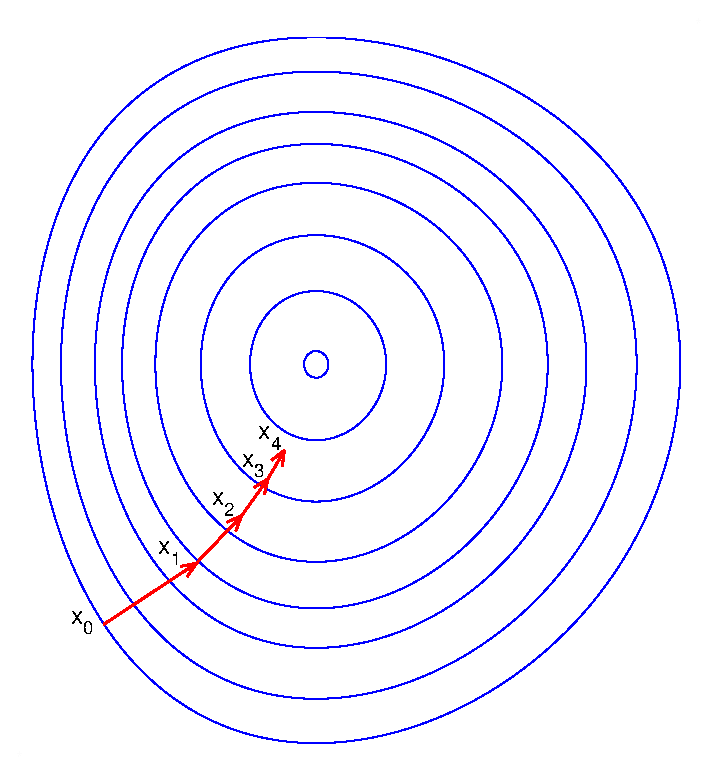
\includegraphics[width=2in]{SourceFiles/plots/Gradient_descent.eps}
\end{center}
\end{frame}

\begin{frame}
\frametitle{ Smoothness and Strong Convexity }

\begin{block}{$\beta$-Smoothness}
$f$ is $\beta$-smooth if:
\begin{equation}
f(y) \leq f(x) + \nabla f(x)^\top(y-x)+ \frac{\beta}{2} ||x - y||_2^2
\end{equation}
\end{block}

\begin{block}{$\alpha$-Strong Convexity}
$f$ is $\alpha$-strongly convex if:
\begin{equation}
f(y) \geq f(x) + \nabla f(x)^\top(y-x) + \frac{\alpha}{2} ||x - y||_2^2
\end{equation}
\end{block}

\begin{block}{Condition number}
The condition number of a $\beta$-Smooth and $\alpha-$Strongly Convex function equals $\kappa = \frac{\beta}{\alpha}$
\end{block}
\end{frame}


\begin{frame}
\frametitle{Gradient Descent convergence rates}


\fontbig

\begin{center}
 \begin{tabular}{||c c ||} 
 \hline
 Function Class  & GD convergence rate \\ [0.5ex] 
 \hline\hline
 $\beta$-Smooth  & $\frac{1 }{t}$  \\ [1ex]
 \hline
 $\beta$-Smooth, $\alpha-$Strongly Convex   & $\exp\left(-\frac{t}{\kappa}\right)$  \\[1ex]
 \hline
\end{tabular}

\end{center}

\begin{block}{Can we do better?}
\onslide<2->Yes!
\end{block}

\end{frame}



\begin{frame}

\frametitle{Nesterov Accelerated Gradient}


\begin{block}{Nesterov Accelerated Gradient (I)}
Nesterov proposed different acceleration schemes that are applicable for different types of function classes. 
\begin{align}
    x_k = y_k - s \nabla f(y_{k-1}) \\
    y_k = x_k + \frac{k-1}{k+2}(x_k - x_{k-1})
\end{align}
\end{block}

\begin{block}{Nesterov Accelerated (II)}

Applicable when $f$ is $\beta$-smooth and $\alpha-$Strongly convex functions
\begin{align}
x_k = y_{k-1} - \frac{1}{\beta} \nabla f(y_{k-1})\\
y_k = x_k + \frac{\sqrt{\kappa} - 1}{\sqrt{\kappa}+1} (x_k - x_{k-1})
\end{align}

\end{block}

\Fontvi
*We can do this also for noneuclidean geometries via Mirror descent \cite{DBLP:journals/ftml/Bubeck15}.  

\end{frame}



\begin{frame}
\frametitle{Nesterov Gradient Descent convergence rates}
\fontbig
\begin{center}


 \begin{tabular}{||c c c c ||} 
 \hline
 Function Class   & GD  &  Nesterov  \onslide<2-> {& Lower bound }\\ [0.5ex] 
 \hline\hline
 $\beta$-S & $\frac{1}{t}$ & \textcolor{blue}{$\frac{1}{t^2}$} & \onslide<2->{ \textcolor{blue}{$\frac{1}{t^2}$} } \\ [1ex]
 \hline
 $\beta$-S, $\alpha-$SC  &  $\exp\left(-\frac{t}{\kappa}\right)$ & \textcolor{red}{$\exp\left(-\frac{t}{\sqrt{\kappa}}  \right)$} & \onslide<2-> {\textcolor{red}{ $\exp\left(-\frac{t}{\sqrt{\kappa}}  \right)$} }\\ [1ex]
 \hline
\end{tabular}



\end{center}



\begin{block}{Can we do better?}
\onslide<2-> {Not with a first order method \cite{DBLP:journals/ftml/Bubeck15}, \cite{nesterov2004introductory}.}
\end{block}

\end{frame}


\begin{frame}
\frametitle{An ODE for Gradient Descent \cite{su2014differential}}
\begin{block}{Limit of Gradient Descent}
\begin{center}
$x_k \approx X(\overbrace{k s}^{t})$ for the curve $X(t)$: \\
\begin{align*}
\begin{rcases*}
    x_k &= x_{k-1} - s \nabla f(x_{k-1}) \\
\end{rcases*} \overset{s \to 0}{\longrightarrow} \dot{X} = - \underbrace{\nabla f(X)}_{``force"}
\end{align*}
\end{center}
\end{block}

\begin{block}{Lyapunov Functional (Weakly Convex) -- \cite{su2014differential}}
$\textcolor{red}{t} (f(X(t)) - f(x^*)) + \frac{1}{2}||X(t)-x^*||^2 \implies f(X(t))-f(x^*) \lesssim \mathcal{O}(\frac{1}{\textcolor{red}{t}})$
\end{block}

\begin{block}{Lyapunov Functional (Strongly Convex) -- Us!}
$e^{- \textcolor{red}{\alpha} t} (f(X(t)) - f(x^*)) + \frac{1}{2}||X(t)-x^*||^2) \implies f(X(t))-f(x^*) \lesssim \mathcal{O}(e^{-\textcolor{red}{\alpha} t})$
\end{block}


\end{frame}


\begin{frame}
\frametitle{An ODE for Nesterov Acceleration (I) \cite{su2014differential}}
\begin{block}{Limit of ``Accelerated" Gradient Descent (for Weakly Convex $f$)}
\begin{center}
$x_k \approx X(\overbrace{k\sqrt{s}}^{t})$ for the curve $X(t)$: \\
\begin{align*}
\begin{rcases*}
    x_k &= y_{k-1} - s \nabla f(y_{k-1})\\
    y_k &= x_k + \frac{k-1}{k+2} (x_k - x_{k-1}) 
\end{rcases*} \overset{s \to 0}{\longrightarrow} \underbrace{\ddot{X}}_{``mass"} + \underbrace{\frac{3}{t} \dot{X}}_{``damping"} + \underbrace{\nabla f(X)}_{``force"} = 0
\end{align*}
\end{center}
\begin{itemize}
    \item ``Small" $t$: large ``damping" $\implies$ fast decay to equilibrium
    \item "Large" $t$: small "dampling" $\implies$ fast oscillations toward optima
\end{itemize}
\end{block}

\begin{block}{Lyapunov Functional (Weakly Convex) \cite{su2014differential}}
$\textcolor{red}{t^2} (f(X(t)) - f(x^*)) + 2||X+t \dot{X}/2 - x^*||_2^2 \implies f(X(t)) - f(x^*) \lesssim \mathcal{O}(1/\textcolor{red}{t^2})$
\end{block}
\end{frame}

\begin{frame}
\frametitle{An ODE for Nesterov Acceleration (I) \cite{su2014differential}}
Minimizing $f(X_1, X_2) = 0.02 X_1^2 + 0.005 X_2^2$.
\begin{figure}
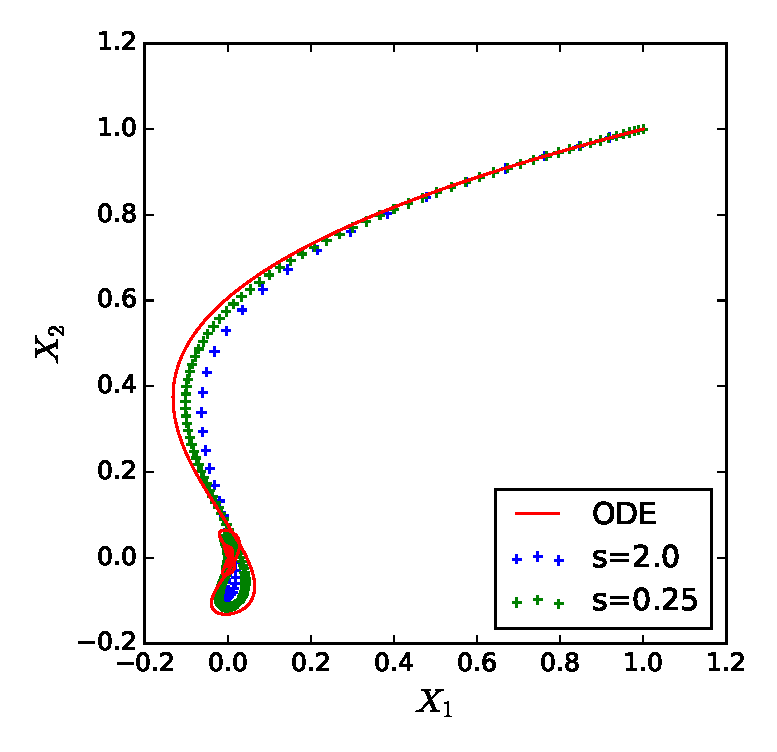
\includegraphics[width=0.6\linewidth]{Experiments/quadratic_traj_compare_annealed.eps}
\caption{}
\end{figure}
\end{frame}

\begin{frame}
\frametitle{An ODE for Nesterov Acceleration (II) Us!}
\begin{block}{Limit of ``Accelerated" Gradient Descent (for Strongly Convex $f$ )}
\begin{center}
$x_k \approx X(\overbrace{k\sqrt{s}}^{t})$ for the curve $X(t)$: \\
\begin{align*}
\begin{rcases*}
    x_k &= y_{k-1} - \overbrace{\frac{1}{\beta}}^{s} \nabla f(y_{k-1})\\
    y_k &= x_k + \frac{\sqrt{\kappa(\beta)}-1}{\sqrt{\kappa(\beta)}+1} (x_k - x_{k-1}) 
\end{rcases*} \overset{s \to 0}{\longrightarrow} \underbrace{\ddot{X}}_{``mass"} + \underbrace{2 \sqrt{\alpha} \dot{X}}_{``damping"} + \underbrace{\nabla f(X)}_{``force"} = 0
\end{align*}
\end{center}
\end{block}


\begin{block}{Lyapunov Functional (Strongly Convex) Us!}
\small{
$e^{\textcolor{red}{\sqrt{\alpha}} t} (f(X(t)) - f(x^*)) + \frac{\alpha}{2} ||X+\frac{1}{\sqrt{\alpha}} \dot{X} - x^*||_2^2 \implies f(X(t)) - f(x^*) \lesssim \mathcal{O}(e^{-\textcolor{red}{\sqrt{\alpha}} t})$}
\end{block}

\end{frame}

\begin{frame}
\frametitle{An ODE for Nesterov Acceleration (II) Us!}
\begin{block}{$f(X) = \frac{\alpha}{2} X^2 \equiv$ Damped Harmonic Oscillator!}
\begin{center}
\vspace{-,25cm}
\begin{align*}
   \ddot{X} + 2 \zeta \sqrt{\alpha} \dot{X} + \alpha X = 0 \implies 
\end{align*}
\vspace{-1cm}
\begin{align*}
   X(t) = \begin{cases}
   & e^{-\zeta \sqrt{\alpha} t} \left( C \cos(\alpha(1-\zeta^2) t+\phi \right) \text{ when } \zeta < 1 \\
   & e^{-\zeta \sqrt{\alpha} t}(A+B t) \text{ when } \zeta = 1 \ \textcolor{red}{ Nesterov \ Coefficient } \\
   & A e^{ -(\sqrt{\alpha}(\zeta - \sqrt{\zeta^2-1})) t}+ B e^{ -(\sqrt{\alpha}(\zeta + \sqrt{\zeta^2-1}) t})   \text{ when } \zeta > 1
   \end{cases}
\end{align*}
\end{center}
\end{block}

\begin{block}{Nesterov ``Momentum" Coefficient \textit{is} Critical Damping }
\begin{itemize}
\end{block}
\end{frame}

\begin{frame}
\frametitle{An ODE for Nesterov Acceleration (II) Us!}
\begin{block}{$f(X) = \frac{\alpha}{2} X^2 \equiv$ Damped Harmonic Oscillator!}
\begin{center}
\vspace{-,25cm}
\begin{align*}
   \ddot{X} + 2 \zeta \sqrt{\alpha} \dot{X} + \alpha X = 0 \implies 
\end{align*}
\vspace{-1cm}
\begin{align*}
   X(t) = \begin{cases}
   & e^{-\zeta \sqrt{\alpha} t} \left( C \cos(\alpha(1-\zeta^2) t+\phi \right) \text{ when } \zeta < 1 \\
   & e^{-\zeta \sqrt{\alpha} t}(A+B t) \text{ when } \zeta = 1 \ \textcolor{red}{ Nesterov \ Coefficient } \\
   & A e^{ -(\sqrt{\alpha}(\zeta - \sqrt{\zeta^2-1})) t}+ B e^{ -(\sqrt{\alpha}(\zeta + \sqrt{\zeta^2-1}) t})   \text{ when } \zeta > 1
   \end{cases}
\end{align*}
\end{center}
\end{block}

\begin{block}{Nesterov ``Momentum" Coefficient \textit{is} Critical Damping }
\begin{figure}
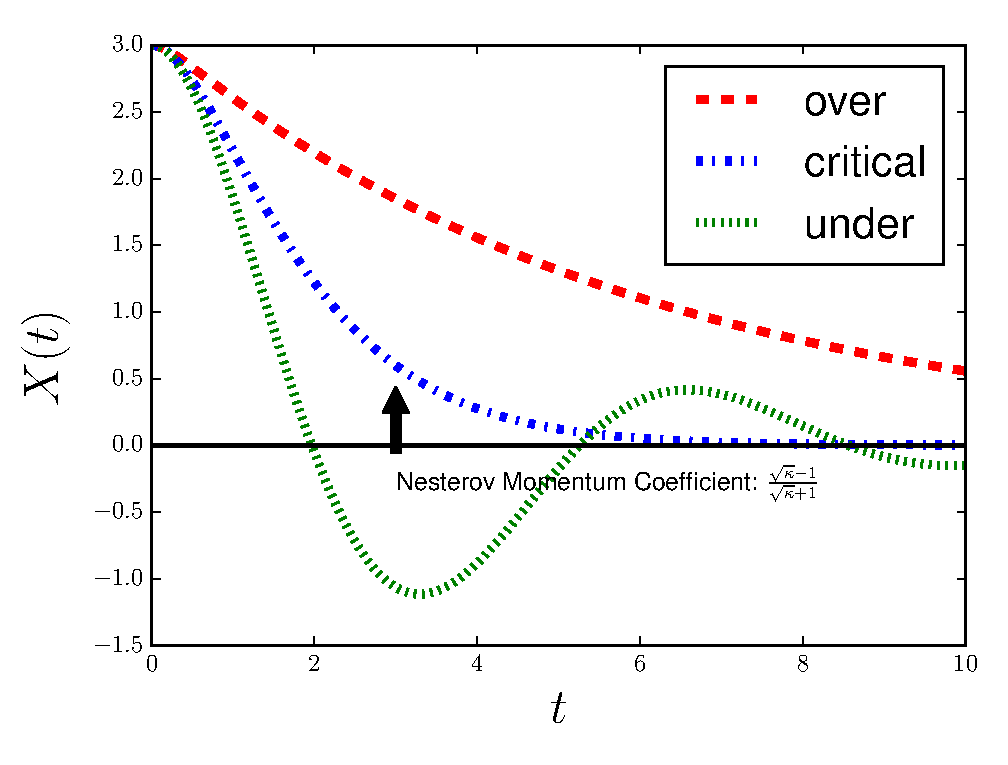
\includegraphics[width=0.4\linewidth]{Experiments/critical_damp_Nesterov.eps}
\caption{}
\end{figure}

\end{block}

\end{frame}



\subsection{Accelerated Mirror Descent}

\begin{frame}
\frametitle{Mirror Descent}
We want to extend these dimension-free convex optimization results to non-Euclidean spaces.
\begin{block}{Projected Gradient Descent}
For the Euclidean projection,
\begin{align*}
x_{k+1} &= \arg\min_{x \in C}\|x_k -\alpha_k \nabla f(x_k) - x\|_2^2 \\
&= \arg\min_{x \in C} <x, \nabla f(x_k)> + \frac{1}{\alpha_k}\frac{\|x - x_k\|_2^2}{2}
\end{align*}
\end{block}
Our Euclidean norm in this case is acting as a distance function for projection.
\begin{block}{Bregman Divergence}
$$D_\Phi(x,y) = \Phi(x) - \Phi(y) - \nabla \Phi(y)^T(x-y)$$
\end{block}
\end{frame}

\begin{frame}
\frametitle{Mirror Descent Algorithm}
\begin{figure}
    \centering
    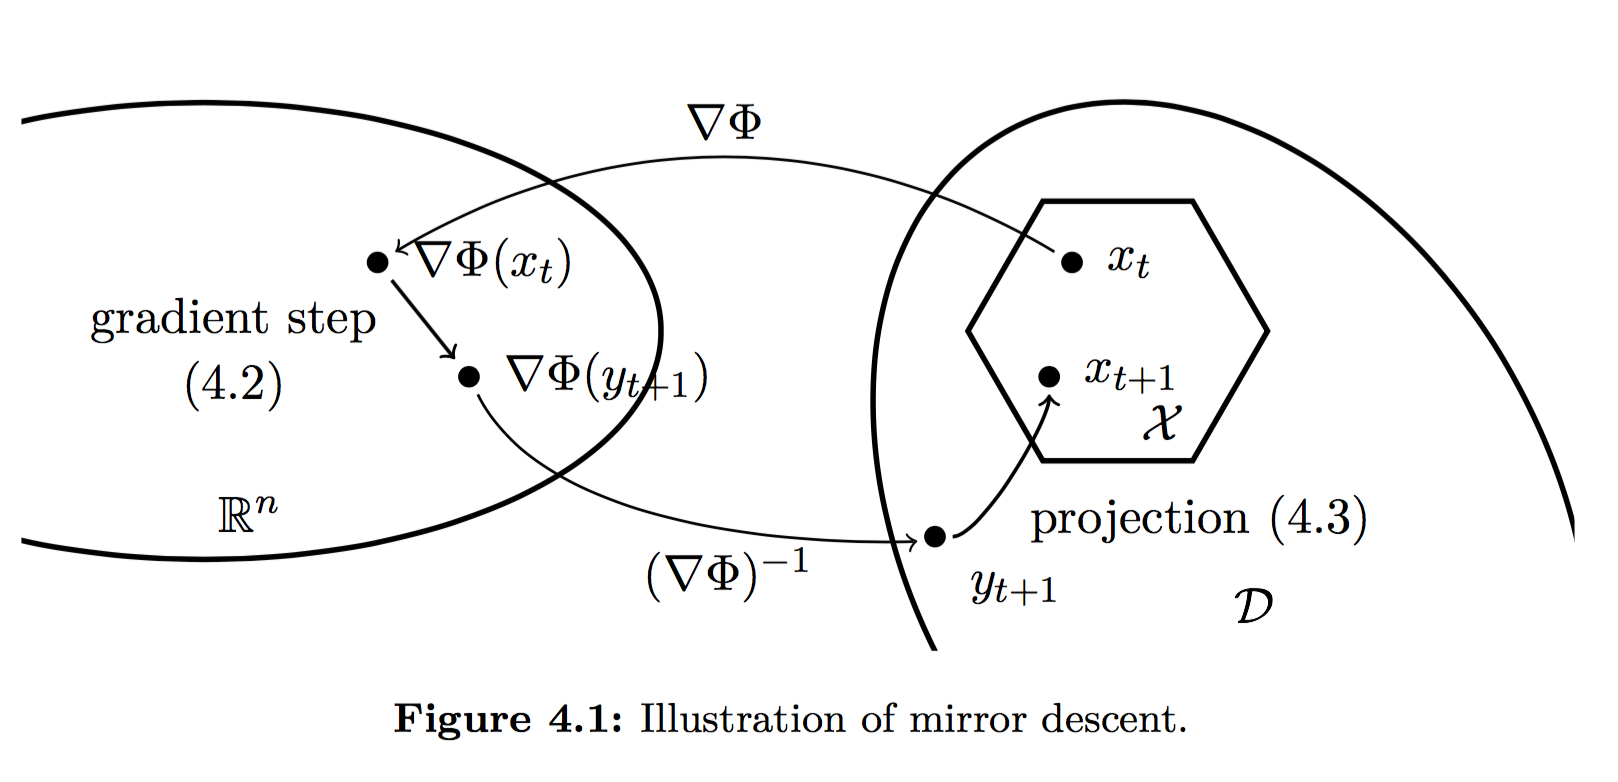
\includegraphics[width=0.9\textwidth]{Images/mda.png}
\end{figure}
\begin{block}{Mirror Descent Update}
$$x_{t+1} = \arg\min_{x \in D} \eta g_t^Tx + D_{\Phi}(x,x_t)$$
\end{block}
\end{frame}

% - Formulate the Lyapanov function
% - A natural non-Euclidean generalization(ball setup, simplex) of the squared Euclidean norm is the Bregman Divergence(KL divergence is an example)

% - Mirror Descent:
\subsection{Mirror Descent ODE}
\begin{frame}
\frametitle{Continuous time mirror ODE}
We generalize, using the Lyapunov function as our starting point
\begin{align*}
\mathcal{E}(t) = \frac{t^2}{r} (f(X) - f^*) + \frac{r}{2} \|X+\frac{t}{r}\dot X - x^* \|^2
\end{align*}
\begin{block}{Generalized Lyapunov}
\begin{align*}
V(X(t),Z(t),t) = \frac{t^2}{r} (f(X(t)) - f^*) + r D_{\psi^*} (Z(t), z^*) 
\end{align*}
\end{block}
chose dynamics $\dot Z = -\frac{t}{r} \nabla f(X)$, and also $\nabla \psi^*(Z) = X + \frac{t}{r} \dot X$ 
\begin{block}{Accelerated Mirror ODE}
\begin{align*}
\dot X = \frac{r}{t} (\nabla \psi^*(Z) - X),\quad \dot Z = -\frac{t}{r} \nabla f(X)
\end{align*}
\end{block}
\end{frame}

\begin{frame}
\frametitle{Accelerated Mirror Descent Algorithm}
\begin{block}{(Forward/Backwards) Euler Method}
\begin{align*} x_{k+1}  &= \lambda_k \nabla \psi^*(z_k) + (1-\lambda_k) x_{k}\\
z_{k+1}& = z_k -\frac{ks}{r} \nabla f(x_{k+1}) 
\end{align*}
If we do something special ** with $\psi$ and $\psi^*$ we can recover that for $\tilde z_{k+1} = \nabla \psi^*(z_{k+1} )$
\[\tilde z_{k+1} = \argmin_{x\in\mathcal{X}} \frac{ks}{r} \langle \nabla f(x_{k+1}), x \rangle + D_\psi (x, \tilde z_k)\]
\end{block}
Modified Lyapunov function
\begin{block}{Proposed Discretization}
\[\tilde x_k = \argmin_{x\in\mathcal X} \gamma s \langle \nabla f(x_k), x \rangle + R(x,x_k) \]
\end{block}
\end{frame}

\section{Plots}
\begin{frame}
\frametitle{Numerical Experiments}
Simplex constrained problems, list mirror map and divergence

figure of quadractic plots
\end{frame}

\begin{frame}
\frametitle{Numerical Experiments}
Simplex constrained problems, list mirror map and divergence

figure of log-sum-exp plots and diverging
\end{frame}

\begin{frame}[t, allowframebreaks]
\frametitle{References}
\footnotesize{
\bibliographystyle{amsalpha}
\bibliography{refs.bib}
\cite{*}}
\end{frame}


\end{document}

